\documentclass[a4paper,12pt]{article} 

\usepackage[top = 2.5cm, bottom = 2.5cm, left = 2.5cm, right = 2.5cm]{geometry} 

\usepackage[T1]{fontenc}
\usepackage[utf8]{inputenc}
\usepackage{amsmath}
\usepackage{multirow}
\usepackage{booktabs} 
\usepackage{tikz}
\usepackage{float,graphicx} 
\usepackage{amssymb} 
\usepackage{pdfpages}
\usepackage{adjustbox}
\usepackage{setspace}
\setlength{\parindent}{0in}

\usepackage{float}

\usepackage{fancyhdr}
\usepackage{enumerate}


\pagestyle{fancy} 
\fancyhf{}
\lhead{\footnotesize PR \& ML: Blatt 4}
\rhead{\footnotesize F. Freter, E. Kirchberger, S. Symhoven \& J. Wustl} %<---- Fill in your lastnames.

\cfoot{\footnotesize \thepage} 

\begin{document}

\thispagestyle{empty} 

\begin{tabular}{p{15.5cm}} 
{\large \bf Pattern Recognition und Machine Learning} \\
Hochschule München \\ Sommersemester 2023  \\ Prof. Dr.-Ing. Claudius Schnörr \\
\hline 
\\
\end{tabular} 

\vspace*{0.3cm} 

\begin{center} 
	{\Large \bf Blatt 4} 
	\vspace{2mm}
	

	{\bf F. Freter, E. Kirchberger, S. Symhoven \& J. Wustl} 
		
\end{center}  

\vspace{0.4cm}

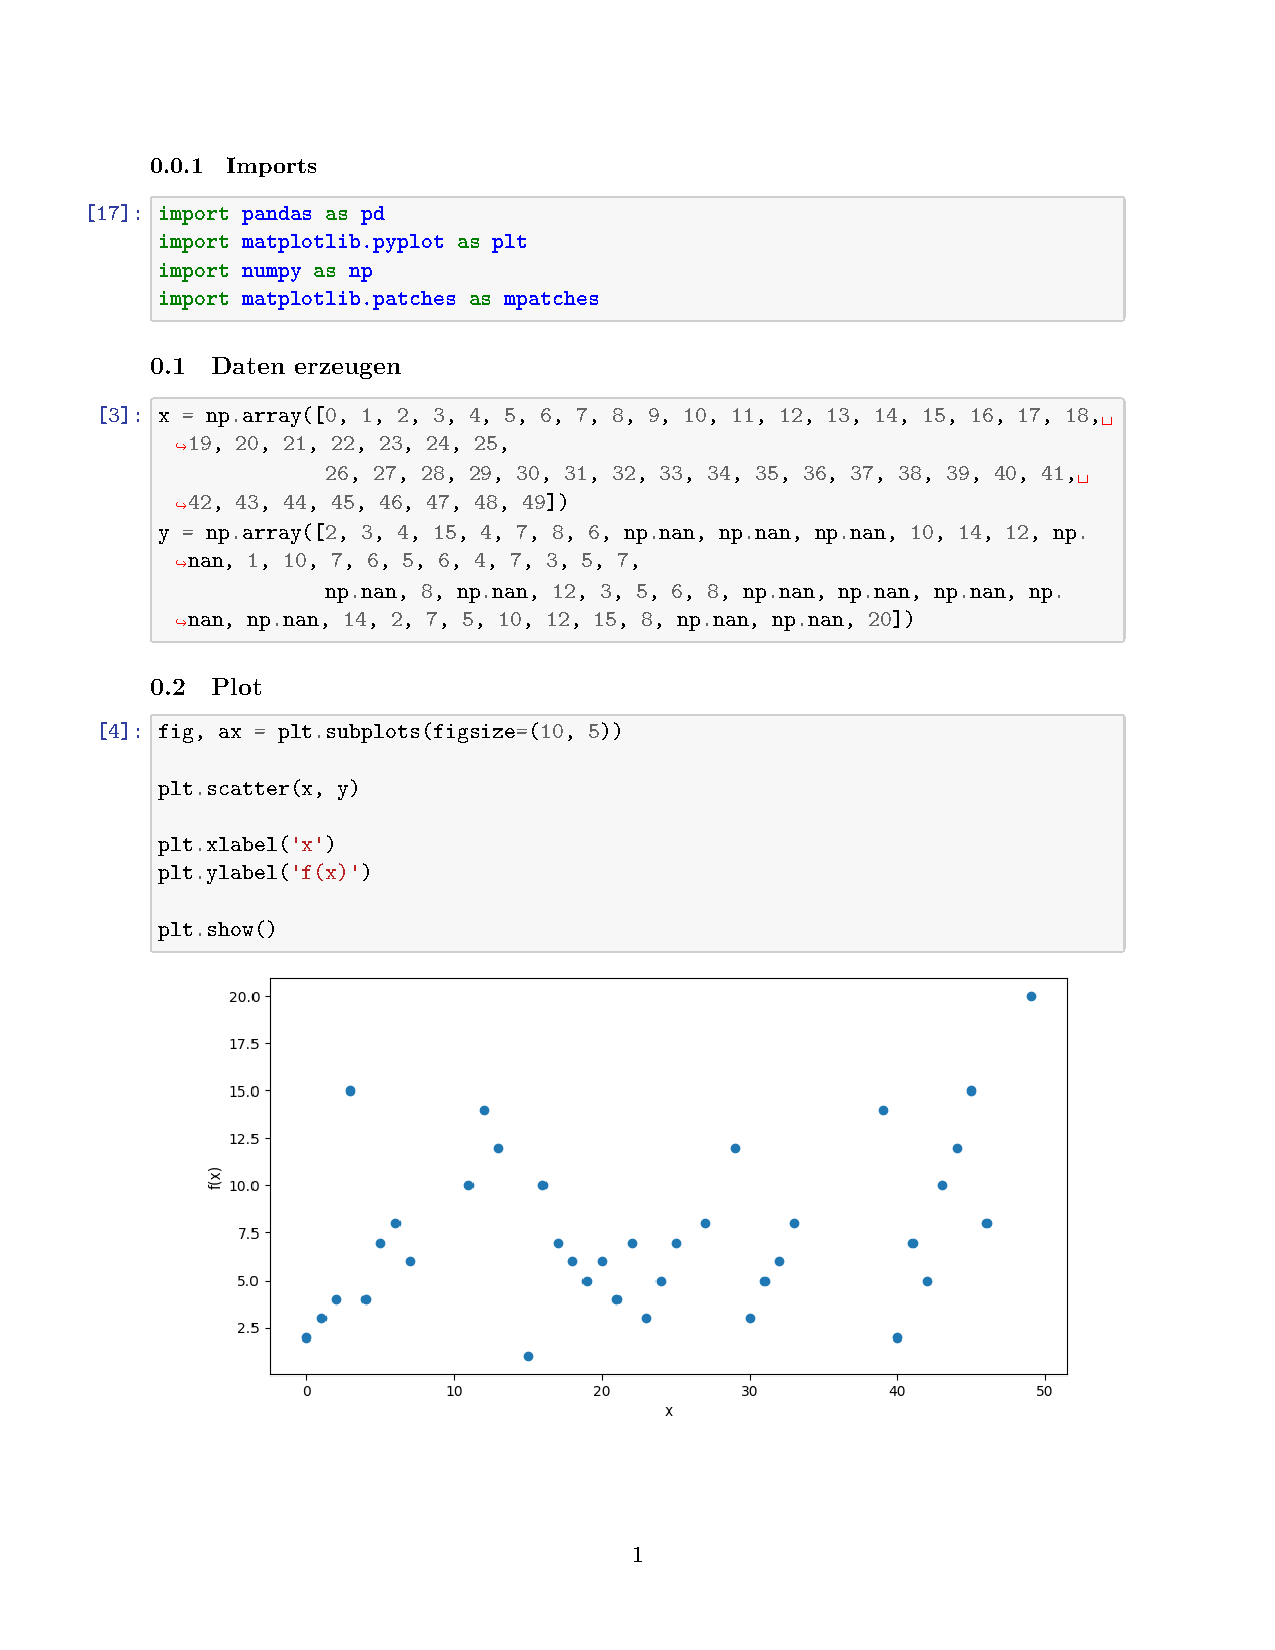
\includepdf[pages=1,pagecommand=\section*{Aufgabe 1/2: Lineare Regression}]{aufgabe-1-2.pdf}
\includepdf[pages={2-}]{aufgabe-1-2.pdf}

\section*{Aufgabe 3: Support Vektor Maschinen}

\subsection*{SVM-Klassifikation:}

\begin{enumerate}

	\item Der Vektor $y$ repräsentiert die Klassenzuordnungen der Trainingsdaten in einem SVM-Klassifikator. 
		In diesem Fall werden Muster der Klasse 1 mit dem Wert 1 gekennzeichnet und Muster der Klasse 2 mit dem Wert -1 gekennzeichnet. 
		Die Reihenfolge der Elemente im Vektor $y$ entspricht der Reihenfolge der entsprechenden Muster in den Datenvektoren $x_1$ bis $x_7$.
		
		\[ y= \begin{pmatrix} -1 & 1 & 1 & -1 & 1 & -1 & -1 \end{pmatrix}^T \]
	
	
	\item
		\begin{figure}[H]
			\centering
			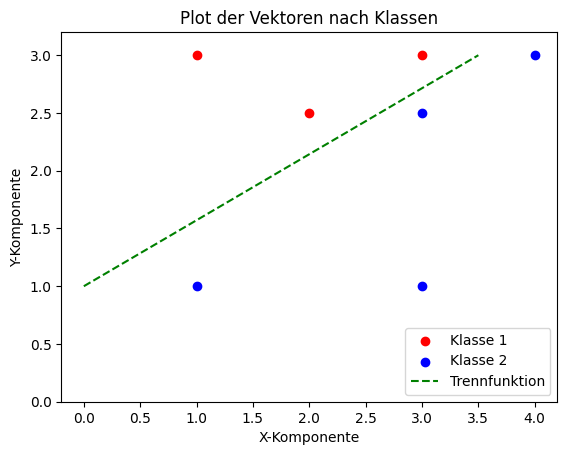
\includegraphics[width = .7\linewidth]{aufgabe-3-2.png}
	  	\end{figure}

		Ja, es handelt sich dabei um eine linear trennbare Problemstellung. Diese kann über zwei Punkte 
		$a=\begin{pmatrix} 0 \\ 1 \end{pmatrix}$ und $b=\begin{pmatrix} 3.5 \\ 3 \end{pmatrix}$ definiert werden 
		und maximiert den Rand zwsichen den beiden Klassen.  
	

	\item 
	
	Um den Gewichtungsvektor w zu berechnen, verwenden wir normalerweise den Ansatz der Support Vector Machine und die Methode der Lagrange-Multiplikatoren. 
	Der Gewichtungsvektor w wird während des Trainingsprozesses der SVM bestimmt und hängt von den Datenpunkten und den Lagrange-Multiplikatoren ab.

	In unserer zeichnerischen Lösung basierend auf den Punkten $a$ und $b$, haben wir bereits eine Trennfunktion definiert. 
	Die Koeffizienten der Geradengleichung, die die beiden Punkte $a$ und $b$ verbindet, bestimmen die Parameter der linearen Trennfunktion:

	Der Schwellenwert $b$ ist der y-Achsenabschnitt und somit die zweite Komponente von dem Punkt $a$.
	
	\[b = 1\]
	
	Der Gewichtungsvektor $w$ der linearen Trennfunktion wird berechnet als:

	\[w = b - a = \begin{pmatrix} 3.5 \\ 3 \end{pmatrix} - \begin{pmatrix} 0 \\ 1 \end{pmatrix} = \begin{pmatrix} 3.5 \\ 2 \end{pmatrix}\]



	\item Daraus ergeben sich die Support-Vektorn $x_2$, $x_5$, $x_6$ und $x_7$.
	
	\item
	\begin{align*}
		\langle w, x \rangle &= \sum_{x_i \in \text{SVs}} \alpha_i y_i K(x, x_i) \\
			&= 8.23 \cdot K(x, x_2) + 0.95 \cdot K(x, x_5) - 8.23 \cdot K(x, x_6) - 0.95 \cdot K(x, x_7) \\
			&= 8.23 \cdot \left( \begin{pmatrix} x_1 & x_2 \end{pmatrix} \cdot  \begin{pmatrix} 3 \\ 3 \end{pmatrix} + 1 \right) + 0.95 \cdot \left(\begin{pmatrix} x_1 & x_2 \end{pmatrix} \cdot \begin{pmatrix} 2 \\ 2.5 \end{pmatrix} + 1 \right) \\ &- 8.23 \cdot \left( \begin{pmatrix} x_1 & x_2 \end{pmatrix} \cdot \begin{pmatrix} 3 \\ 2.5 \end{pmatrix} + 1 \right) - 0.95 \cdot \left( \begin{pmatrix} x_1 & x_2 \end{pmatrix} \cdot \begin{pmatrix} 4 \\ 3 \end{pmatrix} + 1 \right) \\
			&= 8.23 \cdot \left( 3x_1 + 3x_2 + 1\right) + 0.95 \cdot \left( 2x_1 + 2.5x_2 + 1\right) \\ &- 8.23 \cdot \left( 3x_1 + 2.5x_2 + 1\right) - 0.95 \cdot \left( 4x_1 + 3x_2 + 1\right) \\
			&= -1.9x_1 + 3.64x_2
		\end{align*}

	\begin{align*}
		w^* &= \sum_{i=1}^7 \alpha_i^* y_i x_i \\
			&= (8.23 \cdot 1 \cdot x_2) + (0.95 \cdot 1 \cdot x_5) + (8.23 \cdot (-1) \cdot x_6) + (0.95 \cdot (-1) \cdot x_7) \\
			&= (8.23 \cdot 1 \cdot \begin{pmatrix} 3 \\ 3 \end{pmatrix}) + (0.95 \cdot 1 \cdot \begin{pmatrix} 2 \\ 2.5 \end{pmatrix}) + (8.23 \cdot (-1) \cdot \begin{pmatrix} 3 \\ 2.5 \end{pmatrix}) + (0.95 \cdot (-1) \cdot \begin{pmatrix} 4 \\ 3 \end{pmatrix}) \\
			&= 8.23 \cdot \begin{pmatrix} 3 \\ 3 \end{pmatrix} + 0.95 \cdot \begin{pmatrix} 2 \\ 2.5 \end{pmatrix} - 8.23 \cdot \begin{pmatrix} 3 \\ 2.5 \end{pmatrix} - 0.95 \cdot \begin{pmatrix} 4 \\ 3 \end{pmatrix} \\
			&= \begin{pmatrix} -1.9 \\ 3.64 \end{pmatrix}
	\end{align*}

	\item
	
	$i = 2$:
	\begin{align*}
		\alpha_2 \left[(\langle w, x_2 \rangle + b) \cdot y_2 - 1 \right] &= 0 \\
		8.23 \left[((-1.9 \cdot 3 + 3.64 \cdot 3) + b) \cdot 1 - 1 \right] &= 0 \\
		b_2 &= -4.22
	\end{align*}

	$i = 5$:
	\begin{align*}
		\alpha_5 \left[(\langle w, x_5 \rangle + b) \cdot y_5 - 1 \right] &= 0 \\
		0.95 \left[((-1.9 \cdot 2 + 3.64 \cdot 2.5) + b) \cdot 1 - 1 \right] &= 0 \\
		b_5 &= -4.3
	\end{align*}

	$i = 6$:
	\begin{align*}
		\alpha_6 \left[(\langle w, x_6 \rangle + b) \cdot y_6 - 1 \right] &= 0 \\
		8.23 \left[((-1.9 \cdot 3 + 3.64 \cdot 2.5) + b) \cdot (-1) - 1 \right] &= 0 \\
		b_6 &= -4.4
	\end{align*}

	$i = 7$:
	\begin{align*}
		\alpha_7 \left[(\langle w, x_7 \rangle + b) \cdot y_7 - 1 \right] &= 0 \\
		0.95 \left[((-1.9 \cdot 4 + 3.64 \cdot 3) + b) \cdot (-1) - 1 \right] &= 0 \\
		b_7 &= -4.32
	\end{align*}
	
	Gemittelt über alle Support-Vektoren ist $b$:

	\[b = \frac{1}{4} \biggl(-4.22 + (-4.3) + (-4.4) + (-4.32)\biggr) = -4.31 \]
	
	\item

	\begin{align*}
		f(x_s) &= sign(\langle w, x_s\rangle + b) \\
			&= sign(-1.9 \cdot 2 + 3.64 \cdot 2 - 4.31) \\
			&= sign(-0.83) \\
			&= -1 
	\end{align*}

	Der Punkt $x_s$ ist somit als Klasse 2 zu klassifizieren.
\end{enumerate}



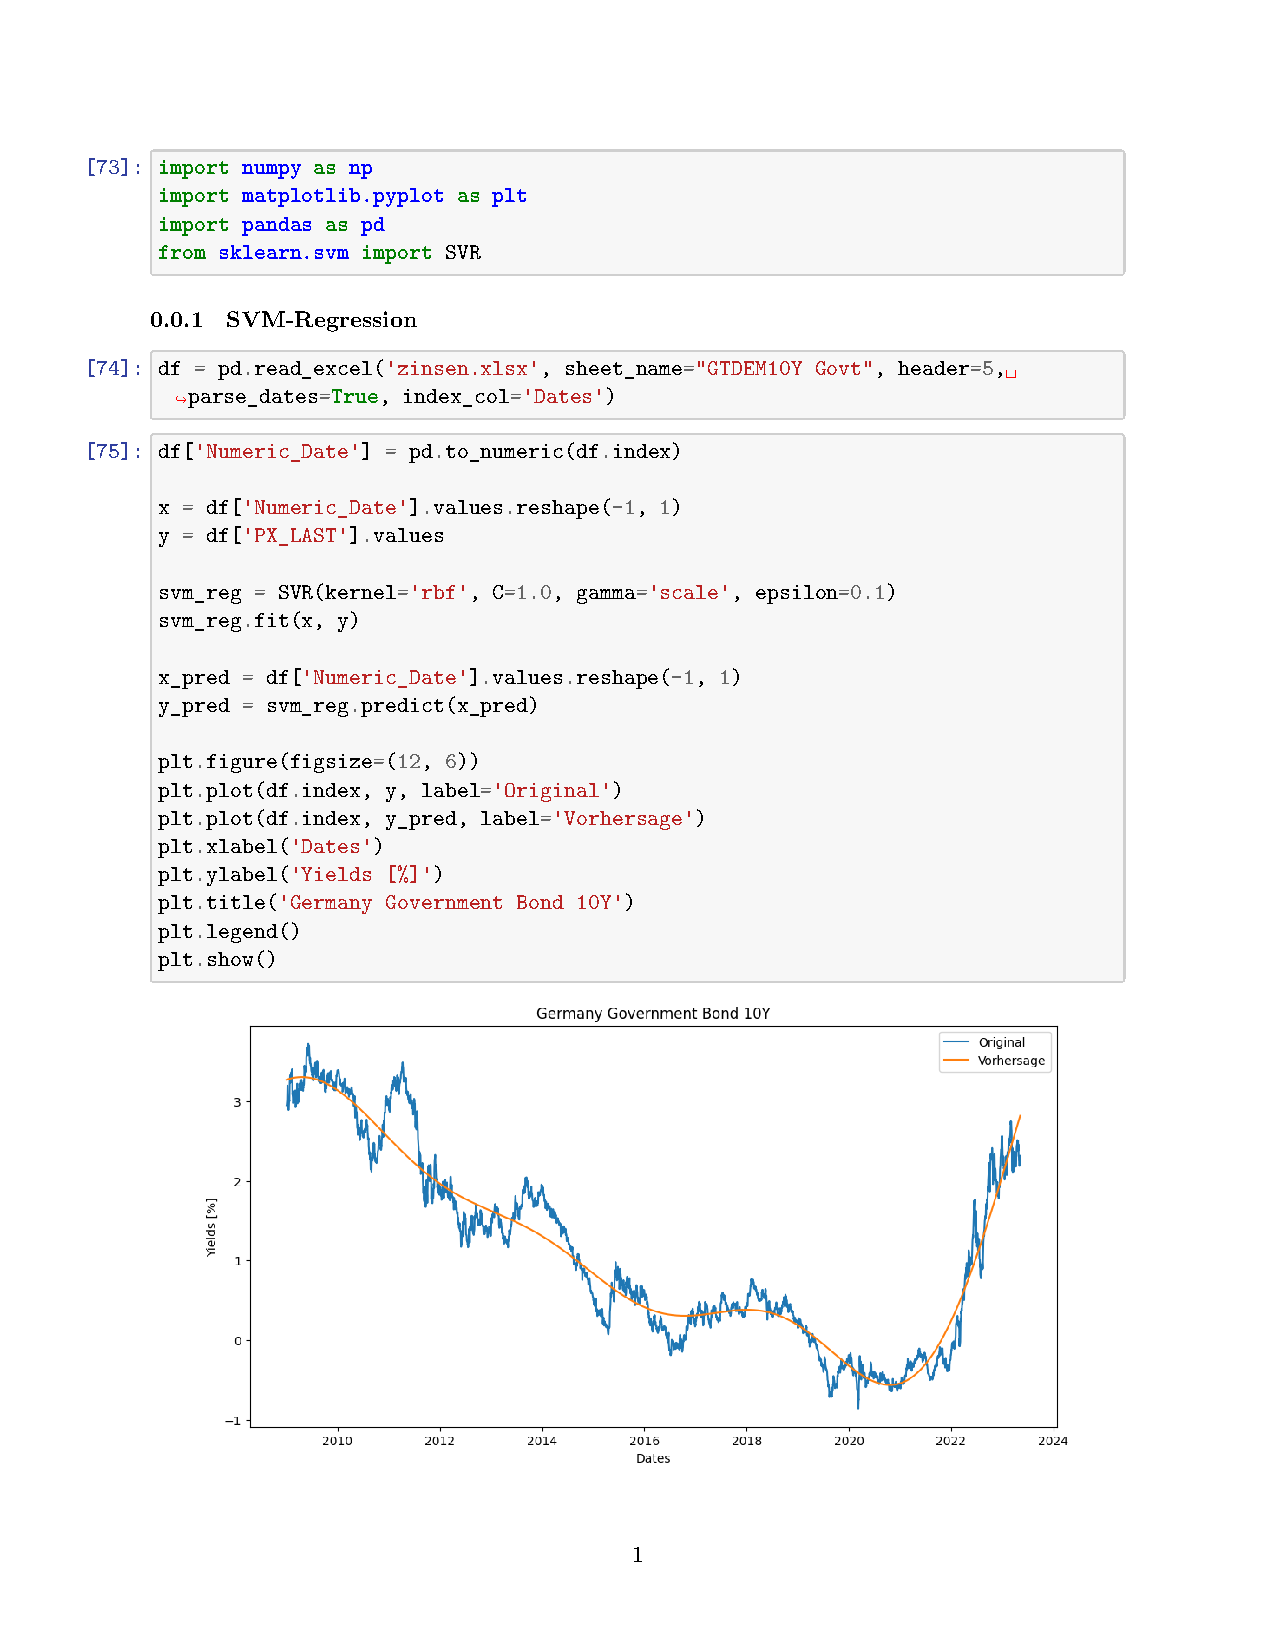
\includepdf[pages=1,pagecommand=\subsection*{SVM-Regression:}]{aufgabe-3-2.pdf}

Parameter $\mathcal{C}$:\\

Der Parameter $\mathcal{C}$ steuert die Straffunktion in der SVM-Regression. 
Ein kleinerer Wert von $\mathcal{C}$ führt zu einer größeren Strafe für Datenpunkte, 
die gegen den Rand der Entscheidungsgrenze verstoßen. Ein größerer Wert von $\mathcal{C}$ erlaubt eine 
größere Flexibilität der Entscheidungsgrenze, um mehr Datenpunkte zu umfassen. \\




Parameter $\sigma$:\\

Der Parameter $\sigma$ steuert die Reichweite des Einflusses jedes 
einzelnen Trainingspunkts. Ein kleinerer Wert von gamma führt zu einer größeren Reichweite 
und einer glatteren Entscheidungsgrenze. Ein größerer Wert von $\sigma$ führt zu einer 
geringeren Reichweite und einer stärkeren Anpassung an einzelne Trainingspunkte. \\



Parameter $\varepsilon$:\\

Der Parameter $\varepsilon$ bestimmt die Breite des Epsilon-Schlauchs, 
der die Toleranz für die Vorhersageabweichung von den Trainingsdaten darstellt. 
Ein kleinerer Wert von $\varepsilon$ erlaubt weniger Toleranz und erfordert eine 
genauere Anpassung an die Trainingsdaten. 
Ein größerer Wert von $\varepsilon$ erlaubt eine größere Toleranz und ermöglicht eine 
gewisse Flexibilität in der Vorhersage.

\end{document}
